\chapter{Chapter 12}

\begin{battle}[0:27]{Anavatapta Warmech}
	\begin{itemize}
		\item Down+A
		\item Side+A
		\item \textit{If Chain died:}
		      \begin{itemize}
			      \item Side+A until \stagger
			      \item Y - Zantetsuken
		      \end{itemize}
		\item \textit{Otherwise:}
		      \begin{itemize}
			      \item Side+A, waiting for the meter to reset before triggering
			      \item Down+A when 18 Gestalt points remain
			      \item Side+A, waiting for meter to reset before triggering.
			      \item If you didn't stagger with the 12 point Gestalt, immediately Y - Zantetsuken
		      \end{itemize}
	\end{itemize}
\end{battle}

\decep{the maze}{the circling Bulwarker}

\textbf{Deceptisol} between the two battle zones, don't cancel.

\begin{menu}
	\begin{itemize}
		\paradigm
		\begin{itemize}
			\item Battle Team
			      \begin{itemize}
				      \item Switch Lightning with Vanille (1 $\leftrightarrow$ 3)
				      \item Switch Lightning with Sazh (3 $\leftrightarrow$ 4)
			      \end{itemize}
			\item Make the second paradigm default
			\item \textit{If you don't have a deceptisol for this fight:}
				\begin{itemize}
					\item Make two Mystic Towers (\rav/\sen/\rav) and set one of them as default.
				\end{itemize}
		\end{itemize}
	\end{itemize}
\end{menu}

\renewcommand{\second}{[2] Relentless Assault (\rav/\rav/\com)}

\begin{battle}[0:14]{Bulwarker \& Sanctum Seraph x2 | DECEPTISOL}
	\begin{itemize}
		\item \second
		      \begin{itemize}
			      \item Quake
			      \item Fira-Aerora
			      \item Summon
			      \item Repeat
			      \item X - Gestalt
			      \item Y - Gaian Salvo
		      \end{itemize}
	\end{itemize}
	\itemdrop{0.38}{Aegisol}
\end{battle}
\renewcommand{\fourth}{[4] Mystic Tower (\rav/\sen/\rav)}
\renewcommand{\fifth}{[5] Mystic Tower (\rav/\sen/\rav)}
\begin{battle}[1:00]{Bulwarker \& Sanctum Seraph x2 | NO DECEPTISOL}
	\begin{itemize}
		\item \fourth
		      \begin{itemize}
		      		\item Target Bulwarker
			      \item Quake
			      \item Fira-Aerora
		      \end{itemize}
		\item \fifth
			\begin{itemize}
				\item Repeat x2
				\item Quake
				\item Summon
				\item Repeat
			\end{itemize}
		\item \fourth
			\begin{itemize}
				\item Repeat
				\item X - Gestalt
				\item B - Force Blasters
				\item Y - Gaian Salvo
			\end{itemize}
	\end{itemize}
	\itemdrop{0.38}{Aegisol}
\end{battle}
\vfill
\begin{menu}
	\begin{itemize}
		\crystarium
		\begin{itemize}
			\item Vanille
			      \begin{itemize}
				      \item Commando
				            \begin{itemize}
					            \item 11 nodes, Ruin
				            \end{itemize}
				      \item Medic
				            \begin{itemize}
					            \item Right 2, Accessory
					            \item 6 nodes left 1, Magic +22
				            \end{itemize}
			      \end{itemize}
			\item Snow
			      \begin{itemize}
				      \item Ravager
				            \begin{itemize}
					            \item 5 nodes down 2, Accessory
				            \end{itemize}
				      \item Sentinel
				            \begin{itemize}
					            \item 12 nodes, ATB segment
				            \end{itemize}
			      \end{itemize}
			\item Sazh
			      \begin{itemize}
				      \item Ravager
				            \begin{itemize}
					            \item 14 nodes,  HP +100
				            \end{itemize}
			      \end{itemize}
		\end{itemize}
		\equip
		\begin{itemize}
			\item Snow
			      \begin{itemize}
				      \item Blank $\rightarrow$ Warrior's Wristband Lv. 8
			      \end{itemize}
			\item Vanille
			      \begin{itemize}
				      \item Diamond Bangle $\rightarrow$ Silver Bangle
				      \item Blank $\rightarrow$ Black Belt *
			      \end{itemize}
			\item Lightning
			      \begin{itemize}
				      \item Optimize Balanced
				      \item Shaman's Mark $\rightarrow$ Tetradic Tiara
			      \end{itemize}
		\end{itemize}
		\paradigm
		\begin{itemize}
			\item \paradigmdeck{%
				      \paradigmline{Vanille}{Snow}{Sazh}}%
			      {\paradigmline{(\com)}{(\com)}{\com}}%
			      {\paradigmline[2]{\textit{(\com)}}{\textit{(\com)}}{\textit{\com}}}%
			      {\paradigmline{(\sab)}{\sen}{\syn}}%
			      {\paradigmline{\med}{\rav}{[\syn]}}%
			      {\paradigmline{\med}{\rav}{[\rav]}}%
			      {\paradigmline{[\rav]}{\rav}{\rav}}
			\item Switch Vanille with Sazh (1 $\leftrightarrow$ 3)
		\end{itemize}
	\end{itemize}
\end{menu}

\renewcommand{\first}{[1] Cerberus (\com/\com/\com)}
\renewcommand{\second}{[2] Cerberus (\com/\com/\com)}
\renewcommand{\third}{[3] Premeditation (\syn/\sen/\sab)}
\renewcommand{\fourth}{[4] Coordination (\syn/\rav/\med)}
\renewcommand{\fifth}{[5] Thaumaturgy (\rav/\rav/\med)}
\renewcommand{\sixth}{[6] Tri-Disaster (\rav/\rav/\rav)}

\begin{battle}[0:53]{Behemoth King}
	\begin{itemize}
		\item \second
		      \begin{itemize}
			      \item Blitz, \rav-buffer into
		      \end{itemize}
		\item \sixth
		      \begin{itemize}
			      \item Fire x4
		      \end{itemize}
		\item \fourth
		      \begin{itemize}
			      \item Auto-support Sazh (Haste)
			      \item Auto-support Vanille (Haste)
		      \end{itemize}
		\item \fifth \textit{if anyone is in red health else} \sixth
		      \begin{itemize}
			      \item Repeat until 350-400\% Chain
		      \end{itemize}
		\item \third
		      \begin{itemize}
			      \item Bravery-Enfire Sazh
			      \item Repeat Snow
			      \item Faith-Enfire Vanille if waiting for Deprotect and Imperil
			      \item Shift after Deprotect and Imperil
		      \end{itemize}
		\item \second
		      \begin{itemize}
			      \item Blitz-Blitz
		      \end{itemize}
	\end{itemize}
	\itemdrop{0.38}{Aegisol}
\end{battle}
\vfill
\begin{menu}
	\begin{itemize}
		\crystarium
		\begin{itemize}
			\item Sazh
			      \begin{itemize}
				      \item Ravager
				            \begin{itemize}
					            \item Left 1, Cold Blood
				            \end{itemize}
			      \end{itemize}
			\item Snow (Optional)
			      \begin{itemize}
				      \item Commando
				            \begin{itemize}
					            \item 4 nodes, HP+60
				            \end{itemize}
			      \end{itemize}
		\end{itemize}
	\end{itemize}
\end{menu}

\decep{battle zone}{big dog}
\textbf{Deceptisol} when the bird falls through the ceiling, don't cancel it.

\begin{battle}[1:31]{Proudclad 1}
	\begin{itemize}
		\item \second
		      \begin{itemize}
			      \item Blitz-execute, \rav-buffer
		      \end{itemize}
		\item \sixth
		      \begin{itemize}
			      \item Fire-Thunder-Fire-Thunder
		      \end{itemize}
		\item \fourth
		      \begin{itemize}
			      \item Bravery-Haste Snow
		      \end{itemize}
		\item \sixth
		      \begin{itemize}
			      \item Repeat
		      \end{itemize}
		\item \fourth
		      \begin{itemize}
			      \item Repeat Sazh
			      \item Faith-Haste Vanille
			      \item Shift after Snow's fifth strike
		      \end{itemize}
		\item \first
		      \begin{itemize}
			      \item Repeat, \rav-buffer the Blitz
		      \end{itemize}
		\item \fifth
		      \begin{itemize}
			      \item Librascope
			      \item Repeat 0-2 spells to get close to stagger, $\sim1\%$ per spell
			      \item Shift after Snow lands
		      \end{itemize}
		\item \sixth
		      \begin{itemize}
			      \item Cold Blood. Shift after Snow's fifth strike
		      \end{itemize}
		\item \fifth
		      \begin{itemize}
			      \item Repeat, shift immediately
		      \end{itemize}
		\item \sixth
		      \begin{itemize}
			      \item Shift after Snow's fifth Strike
		      \end{itemize}
		\item \first
		      \begin{itemize}
			      \item Repeat
			      \item Renew
			      \item Blitz-Blitz, shift after Snow's fifth attack
		      \end{itemize}
		\item \second
		      \begin{itemize}
			      \item Repeat
			      \item Repeat a single Blitz
			      \item Auto-Battle and hope if not dead
		      \end{itemize}
	\end{itemize}
	\itemdrop{0.38}{Deceptisol}
\end{battle}

\begin{menu}
	\begin{itemize}
		\item Snow Adamanchelid:
		      \begin{itemize}
			      \paradigm
			      \begin{itemize}
				      \item Battle Team
				            \begin{itemize}
					            \item Switch Sazh with Snow (1 $\leftrightarrow$ 2)
				            \end{itemize}
				      \item Make the last paradigm the default
			      \end{itemize}
		      \end{itemize}
		\item Lightning Adamanchelid:
		      \begin{itemize}
			      \paradigm
			      \begin{itemize}
				      \item Battle Team
				            \begin{itemize}
					            \item Switch Sazh with Lightning (1 $\leftrightarrow$ 4)
				            \end{itemize}
				      \item Change the second paradigm to Tri-Disaster (\rav/\rav/\rav)
			      \end{itemize}
		      \end{itemize}
	\end{itemize}
\end{menu}

\begin{battle}[0:45]{Adamanchelid (Lightning)}
	\renewcommand{\first}{[1] Solidarity (\com/\sen/\med)}
	\renewcommand{\second}{[2] Tri-Disaster (\rav/\rav/\rav)}
	\begin{itemize}
		\item \first
		      \begin{itemize}
			      \item Attack immediately to dodge first stomp
			      \item Shift in the air
		      \end{itemize}
		\item \second
		      \begin{itemize}
			      \item Strike-Thunder-Thunder-Thunder
			      \item Repeat/Cancel strings to avoid stomps
			      \item Summon when Vanille dies
			      \item Repeat while dodging stomps until 390\% (4 hits), 355\% (5 hits), 345\% (6 hits), 310\% (7 hits)
			      \item X - Gestalt
			      \item If in a Stomp/Quake animation: Down + A - Lightning Strike
			      \item Side + A - Razor Gale until half health and 725\% chain (one less if Zantetsuken Lv. 3)
			      \item Y - Zantetsuken
		      \end{itemize}
	\end{itemize}
	\itemdrop{23.75}{Gold Dust}\itemdrop{ 5}{Scarletite}\itemdrop{ 0.38}{Deceptisol}
\end{battle}

Consult the following chart to determine which chests to get. If you got the Gold Dust, add 15,000 to your gil total. Random drops from Chapter 12 also add to this total, such as: Scarletite (7,000), Incentive Chip (2,500), Credit Chip (500), Chobham Armor (500), Electrolytic Capacitor (160).

\begingroup
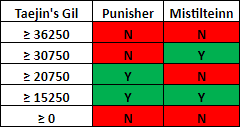
\includegraphics[width=9cm]{./Chapters/gil_pickups.png}
\endgroup

\pickup{Punisher}{forward and to the right if needed}
Push VH+T to the side.
\pickup{Particle Accelerator x6}{on the left side of the glass, then run backwards}
\pickup{Mistilteinn}{in of the long hallway if needed}
\pickup{Power Glove}{up the steps}
\vfill
\ 
\columnbreak

\begin{upgrade}
	\begin{itemize}
		\item Upgrade
		      \begin{itemize}
			      \item Accessories
			            \begin{itemize}
				            \item Power Glove
				                  \begin{itemize}
					                  \item Wicked Fang x41 (3x EXP)
					                  \item Particle Accelerator x6 (*)
				                  \end{itemize}
				            \item Goddess's Favor
				                  \begin{itemize}
					                  \item Particle Accelerator x1 (*)
				                  \end{itemize}
			            \end{itemize}
		      \end{itemize}
		\item Dismantle
		      \begin{itemize}
			      \item Accessories
			            \begin{itemize}
				            \item Goddess's Favor * (Scarletite, Perfume, Ribbon)
				            \item Ribbon (Dusklight Dew x6)
			            \end{itemize}
		      \end{itemize}
		\item Upgrade
		      \begin{itemize}
			      \item Warrior's Wristband * on Snow
			            \begin{itemize}
				            \item Scarletite (Power Glove Lv. 9)
			            \end{itemize}
		      \end{itemize}
	\end{itemize}
\end{upgrade}
	\begin{menu}
		\begin{itemize}
			\crystarium
			\begin{itemize}
				\item Snow
				      \begin{itemize}
					      \item Commando
					            \begin{itemize}
						            \item 11-15 nodes, HP +30 end of stage 7
					            \end{itemize}
				      \end{itemize}
				\item Vanille
				      \begin{itemize}
					      \item Medic
					            \begin{itemize}
						            \item 1 left, Curaja
						            \item 1 Node, Role Level
					            \end{itemize}
				      \end{itemize}
				\item Sazh
				      \begin{itemize}
					      \item Commando
					            \begin{itemize}
						            \item 5 nodes, HP +70
					            \end{itemize}
				      \end{itemize}
			\end{itemize}
			\equip
			\begin{itemize}
				\item Lightning
				      \begin{itemize}
					      \item Unequip all
				      \end{itemize}
				\item Snow
				      \begin{itemize}
					      \item WW Lv 8 $\rightarrow$ Power Glove *
				      \end{itemize}
			\end{itemize}
			\paradigm
			\begin{itemize}
				\item Battle Team
				      \begin{itemize}
					      \item Switch Sazh with Lightning (1 $\leftrightarrow$ 4)
				      \end{itemize}
				\item \paradigmdeck{%
					      \paradigmline{Sazh}{Snow}{Vanille}}%
				      {\paradigmline{\com}{\sen}{\med}}%
				      {\paradigmline{(\rav)}{\rav}{\rav}}%
				      {\paradigmline{(\rav)}{\sen}{(\rav)}}%
				      {\paradigmline{\rav}{\com}{(\com)}}%
				      {\paradigmline{\rav}{\com}{(\rav)}}%
				      {\paradigmline[6]{\textit{(\com)}}{\textit{\com}}{\textit{(\com)}}}
				\item Swap the First and Fourth Paradigms
				\item Swap the Sixth and Second Paradigms
			\end{itemize}
		\end{itemize}
	\end{menu}

Activate \textbf{Ethersol, Fortisol, Aegisol}.
\vfill
\renewcommand{\first}{[1] Aggression (\rav/\com/\com)}
\renewcommand{\second}{[2] Cerberus (\com/\com/\com)}
\renewcommand{\third}{[3] Mystic Tower (\rav/\sen/\rav)}
\renewcommand{\fourth}{[4] Solidarity (\com/\sen/\med)}
\renewcommand{\fifth}{[5] Relentless Assault (\rav/\com/\rav)}
\renewcommand{\sixth}{[6] Tri-Disaster (\rav/\rav/\rav)}
\begin{battle}[2:01]{Proudclad 2}
		\begin{itemize}
			\item \second
			      \begin{itemize}
				      \item Attack-Blitz, \rav-buffer the Blitz into
			      \end{itemize}
			\item \sixth
			      \begin{itemize}
				      \item Libra
				      \item Cold Blood
			      \end{itemize}
			\item \fifth
			      \begin{itemize}
				      \item Repeat
				      \item Shift after Vanille's final attack
			      \end{itemize}
			\item \first
			      \begin{itemize}
				      \item Cold Blood
			      \end{itemize}
			\item \second
			      \begin{itemize}
				      \item Renew
				      \item If Proudclad hits the ground, coordinate attacks to maintain interruption until Launch
				      \item Until stagger is close to ending, Auto-Battle 3 Attacks, alternate with Vanille
				      \item Potion if everyone isn't at max HP
				      \item Attack-Attack-Blitz, \rav-buffer the Blitz
			      \end{itemize}
			\item \third
			      \begin{itemize}
				      \item Auto-Chain one spell
				      \item \textit{Oneiric Maelstrom}:
				            \begin{itemize}
					            \item Renew to prevent Sazh from Launching
					            \item Auto-Chain 2 spells
					            \item Cold Blood
				            \end{itemize}
				      \item \textit{Muon Blaster $\rightarrow$ Oneiric Maelstrom}
				            \begin{itemize}
					            \item Renew to prevent Sazh from Launching
					            \item Cold Blood
				            \end{itemize}
				      \item \textit{Muon Blaster $\rightarrow$ Muon Blaster}
				            \begin{itemize}
					            \item Cold Blood to prevent Sazh's interruption
				            \end{itemize}
				      \item ATB refresh after Cold Blood starts to maximize Launches
			      \end{itemize}
			\item \fifth
			      \begin{itemize}
				      \item Repeat
				      \item Shift after Vanille's final attack
			      \end{itemize}
			\item \first
			      \begin{itemize}
				      \item Repeat
				      \item If Proudclad lands, ATB refresh Snow's fifth attack
				      \item ATB refresh so that Snow and Vanille finish just after you can control Sazh
			      \end{itemize}
			\item \second
			      \begin{itemize}
				      \item Repeat one Attack
				      \item Blitz-Blitz
				      \item Repeat
			      \end{itemize}
			\item \textit{If unlikely to kill before stagger ends}:
			      \begin{itemize}
				      \item \first
				            \begin{itemize}
					            \item Repeat and Shift immediately
				            \end{itemize}
				      \item \second
				            \begin{itemize}
					            \item Hope and Cry
				            \end{itemize}
			      \end{itemize}
			\item \textit{If Proudclad survives}:
			\item \fourth
			      \begin{itemize}
				      \item Potion if low, Repeat otherwise
				      \item Stagger in [6] or damage in [2] as needed, go back to [4] to heal as needed.
			      \end{itemize}
		\end{itemize}
\end{battle}
\save{1}
\vfill
\ 
\columnbreak